\begin{figure}[t]
\centering
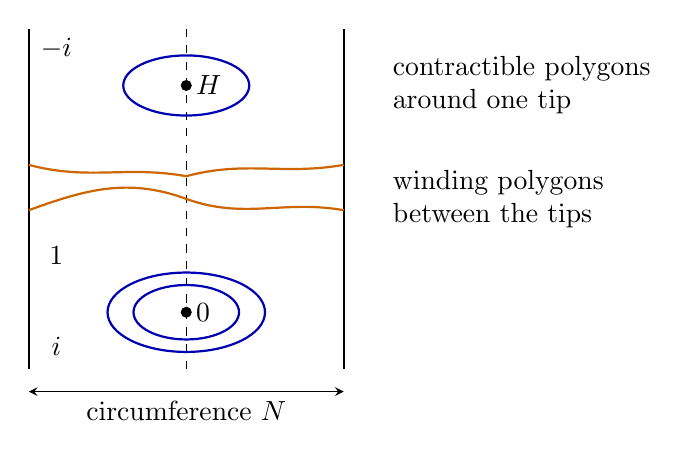
\begin{tikzpicture}[x=1cm,y=.72cm,>=stealth]
\draw[thick] (0,0)--(0,6) (4,0)--(4,6);
\draw[dashed] (2,0)--(2,6);
\fill (2,1) circle(2pt) node[right] {$0$};
\fill (2,5) circle(2pt) node[right] {$H$};
\node at (.35,.4) {$i$};
\node at (.35,2) {$1$};
\node at (.35,5.65) {$-i$};
\draw[blue!70!black,thick] (2,1) ellipse(.67 and .48);
\draw[blue!70!black,thick] (2,1) ellipse(1 and .7);
\draw[blue!70!black,thick] (2,5) ellipse(.8 and .53);
\draw[orange!80!black,thick] (0,2.8) to[out=20,in=160] (2,3) to[out=-20,in=170] (4,2.8);
\draw[orange!80!black,thick] (0,3.6) to[out=-15,in=170] (2,3.4) to[out=15,in=190] (4,3.6);
\draw[<->] (0,-.4)--(4,-.4) node[midway,below] {circumference $N$};
\node[align=left,anchor=west] at (4.5,5) {contractible polygons\\around one tip};
\node[align=left,anchor=west] at (4.5,3) {winding polygons\\between the tips};
\end{tikzpicture}
\caption{A schematic fundamental rectangle for the cylinder: its vertical sides are identified. The dashed seam has tips at cuts $0$ and $H$; the labels $i$, $1$, and $-i$ give its twist in the three row regions. The surviving contractible polygons enclose one tip, and the surviving winding polygons separate the tips. Dividing by the winding growth retains the two tip contributions. Curves are schematic and do not represent individual lattice edges.}
\label{fig:seam}
\end{figure}
